\documentclass[ignorenonframetext, professionalfonts, hyperref={pdftex, unicode}]{beamer}

\usetheme{Copenhagen}
\usecolortheme{wolverine}

%Packages to be included

\usepackage[russian]{babel}
\usepackage[utf8]{inputenc}
\usepackage[T1]{fontenc}


\usepackage[orientation=landscape, size=custom, width=16, height=9.75, scale=0.5]{beamerposter}

\usepackage{textcomp}

\usepackage{beamerthemesplit}

\usepackage{ulem}

\usepackage{verbatim}

\usepackage{ucs}


\usepackage{listings}
\lstloadlanguages{bash}

\lstset{escapechar=`,
	extendedchars=false,
	language=sh,
	frame=single,
	tabsize=2, 
	columns=fullflexible, 
%	basicstyle=\scriptsize,
	keywordstyle=\color{blue}, 
	commentstyle=\itshape\color{brown},
%	identifierstyle=\ttfamily, 
	stringstyle=\mdseries\color{green}, 
	showstringspaces=false, 
	numbers=left, 
	numberstyle=\tiny, 
	breaklines=true, 
	inputencoding=utf8,
	keepspaces=true,
	morekeywords={u\_short, u\_char, u\_long, in\_addr}
	}

\definecolor{darkgreen}{cmyk}{0.7, 0, 1, 0.5}

\lstdefinelanguage{diff}
{
    morekeywords={+, -},
    sensitive=false,
    morecomment=[l]{//},
    morecomment=[s]{/*}{*/},
    morecomment=[l][\color{darkgreen}]{+},
    morecomment=[l][\color{red}]{-},
    morestring=[b]",
}

\author[Epam]{{\bf Epam}\\Embedded solutions department}

%\institution[EPAM]{EPAM}
%\logo{\includegraphics[width=1cm]{logo.png}}


\title[Оптимизация и профилирование]{Оптимизация и профилирование в Linux}

\begin{document}


%%%%%%%%%%%%%%%%%%%%%%%%%%%%%%%%%%%%%%%%%%%%%%%%%
%%%%%%%%%% Begin Document  %%%%%%%%%%%%%%%%%%%%%%
%%%%%%%%%%%%%%%%%%%%%%%%%%%%%%%%%%%%%%%%%%%%%%%%%

\begin{frame}
	\frametitle{}
	\titlepage
	\vspace{-0.5cm}
	\begin{center}
	%\frontpagelogo
	\end{center}
\end{frame}

\begin{frame}
	\tableofcontents
%	[hideallsubsections]
\end{frame}



%%%%%%%%%%%%%%%%%%%%%%%%%%%%%%%%%%%%%%%%%   
%%%%%%%%%% Content starts here %%%%%%%%%%
%%%%%%%%%%%%%%%%%%%%%%%%%%%%%%%%%%%%%%%%%

\section{Профилирование: зачем}
\mode<all>{\begin{frame}
 \frametitle{Оптимизация}
 \begin{itemize}
  \item Преждевременная оптимизация -- корень всех зол!
  \pause
  \item Закон Амдала
     \begin{equation*}
        \frac{1}{(1-P)+\alpha P}
     \end{equation*}
  \item Профилирование -- выясним, в каких местах программа проводит больше всего времени
 \end{itemize}
\end{frame}


\begin{frame}
  \frametitle{Методы профилирования}
  \begin{itemize}
    \item Добавление в код дополнительных инструкций (gprof)
      \begin{enumerate}
        \item[Достоинства] Не требуется поддержка ядра
        \item[Недостатки] Рекомпиляция, замедление кода
      \end{enumerate}
    \item Статистическое исследование (oprofile,perf)
      \begin{enumerate}
        \item[Достоинства] Малое вмешательство в процесс, скорость
        \item[Недостатки] Требуется модуль ядра, точность
      \end{enumerate}
    \item Эмуляция процессора для перехвата вызовов (valgrind)
       \begin{enumerate}
         \item[Достоинства] Не требуется рекомпиляция и модули ядра
         \item[Недостатки] Скорость
        \end{enumerate}
    \item Перехват системных и библиотечных вызовов (strace,ltrace)
       \begin{enumerate}
          \item[Достоинства] Нет рекомпиляции, любое ядро
          \item[Недостатки] Недостаточная информативность
       \end{enumerate}
  \end{itemize}
\end{frame}

}

\section{Gprof}
\mode<all>{\begin{frame}[fragile]
 \frametitle{Gprof}
 \begin{itemize}
   \item Компилировать с опцией \texttt{-pg}
\begin{lstlisting}[language=sh]
 gcc -g -pg -o program program.c
\end{lstlisting}
   \item Создается файл gmon.out
   \item Просмотр статистики (плоский профиль, flat profile) 
\begin{lstlisting}[language=sh]
gprof program -p
\end{lstlisting}
    \item Просмотр графа вызовов со статистикой
\begin{lstlisting}[language=sh]
gprof program -q
\end{lstlisting}
    \item Аннотация исходного кода
\begin{lstlisting}[language=sh]
gprof program -A
\end{lstlisting}
 \end{itemize}
\end{frame}

\begin{frame}
  \frametitle{Упражнение}
  \begin{enumerate}
    \item Изменить Makefile для primefactors.c, так, чтобы включить профилирование
    \item Просмотреть информацию профайлером
  \end{enumerate}
\end{frame}

}

\section{Профилирование в valgrind}
\mode<all>{\begin{frame}[fragile]
 \frametitle{Valgrind callgrind}
 \begin{itemize}
  \item Инструмент для профилирования \verb+ --tool=callgrind+
 \end{itemize}
 \begin{center}
  Упражнение
 \end{center}
 \begin{enumerate}
  \item Скомпилировать ту же самую программу с ключами \verb+-g+
  \item Запустить под valgrind
  \item Изучить callgraph и относительное время в функциях
 \end{enumerate}
\end{frame}
}

\section[oprofile]{Статистическое профилирование в oprofile}
\mode<all>{\begin{frame}
 \frametitle{Статистический сбор образцов: общие соображения}
 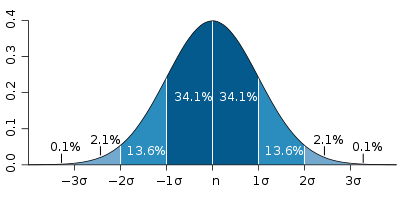
\includegraphics[width=0.7\textwidth]{../../slides/profile/Standard_deviation_diagram.png}
 \begin{itemize}
   \item Распределение Пуассона, в пределе больших $n$ переходящее в нормальное распределение
   \item Ширина распределения $\sim \sqrt{n}$
 \end{itemize}
\end{frame}

\begin{frame}
 \frametitle{Компоненты oprofile}
  \begin{itemize}
    \item Модуль ядра oprofile
    \item Системный демон \texttt{oprofiled}
    \item Программы управления \texttt{opcontrol,opannotate,}
  \end{itemize}
\end{frame}


\begin{frame}[fragile]
 \frametitle{Запуск oprofile: Проверка поддержки в ядре}
 \begin{itemize}
   \item \verb+ grep OPROFILE <configure>+
   \item Где найти \texttt{.configure}
     \begin{itemize}
      \item \texttt{.configure} В исходниках ядра
      \item \verb+/boot/configure-`uname -r`+
      \item \verb+/proc/config.gz+
     \end{itemize}
  \end{itemize}
\end{frame} 


\begin{frame}[fragile]
 \frametitle{Запуск oprofile: Работа}
 \begin{itemize}
  \item \verb+ opcontrol --vmlinux=/boot/vmlinux-3.2.xxx+ 
  \item \verb+ opcontrol --init+
  \item \verb+ opcontrol --start; ./my_program ; opcontrol --dump;  opcontrol --stop+
  \item \verb+ opannotate --source ./my_program +
 \end{itemize}
\end{frame}

\begin{frame}
 \frametitle{Упражнение}
 \begin{enumerate}
  \item Проверить, что в конфигурации ядра есть поддержка oprofile
  \item Скомпилировать программу с \texttt{-g}
  \item Запустить под oprofile
  \item Посмотреть статистику вызовов
  \item Запустить еще раз
  \item Посмотреть статистику еще раз, сравнить
 \end{enumerate}
\end{frame}
}

\section{Анализ тестового покрытия}
\mode<all>{\begin{frame}[fragile]
 \frametitle{Анализ покрытия кода}
 \begin{itemize}
   \item Флаги gcc: \verb+-fprofile-arcs -ftest-coverage+
   \item Инструмент gcov
 \end{itemize}
\end{frame}
}

\end{document}
